\documentclass[fleqn]{article}
\usepackage[left=1in, right=1in, top=1in, bottom=1in]{geometry}
\usepackage{mathexam}
\usepackage{graphicx}
\usepackage{amsmath, bm}
\usepackage{algorithm}
\usepackage{algorithmic}
\usepackage{listings}
\usepackage{color} 
\definecolor{mygreen}{RGB}{28,172,0} 
\definecolor{mylilas}{RGB}{170,55,241}


\ExamClass{Homework 3}
\ExamName{ECS 231}
\ExamHead{Spring 2016}

\let\ds\displaystyle
$\qquad\qquad\qquad\qquad\qquad\qquad Jianshi\quad Zhang$  $\qquad\qquad\qquad$ SID: 912487753

\hline
\begin{document}
\hline
\newpage
\section{ Algorithms}

\begin{algorithm}
         \caption{Steepest Descent Algorithm}              
         \label{alg1}                         
         \begin{algorithmic}
         \STATE \textbf{1.} Initial  $\bm{x_0} = \bm{0}$;
         \STATE  $\quad$ $k = 0$
         \STATE  $\quad$ $\bm{r_0} = \bm{b} - \bm{A}\bm{x_0}$
        
         
         \STATE \textbf{2.} \bm{While}  $\Vert\bm{r_{k}}\Vert_2 > 10^{-6}\Vert\bm{b}\Vert_2$
         \STATE $\quad$ (1). $\bm{\alpha_k} = \frac{\bm{r_k^T}\bm{r_k}}{\bm{r_k^T}\bm{A}\bm{r_k}}$\\[1ex]
         \STATE $\quad$ (2). $\bm{x_{k+1}} = \bm{x_k} + \bm{\alpha_k}\bm{r_k}$\\[1ex]
         \STATE $\quad$ (3).  $\bm{r_{k+1}} = \bm{b} - \bm{A}\bm{x_{k+1}}$\\[1ex]
         \STATE $\quad$ (4).  $k = k + 1$,
        
         \STATE $\qquad$ \bm{end}
        \end{algorithmic}
\end{algorithm}

\begin{algorithm}
\caption{Conjugate Gradient method}            
         \begin{algorithmic}
         \STATE \textbf{1.} Initial  $\bm{x_0} = \bm{0}$;
         \STATE  $\quad$ $k = 0$
         \STATE  $\quad$ $\bm{r_0} = \bm{b} - \bm{A}\bm{x_0}$
        \STATE  $\quad$ $\bm{p_0} = \bm{r_0}$
        
         
         \STATE \textbf{2.} For $k = 0, 1, \dots$
         \STATE $\quad$ (1). Calculate $\bm{Ap_k} = \bm{A}*\bm{p_k}$ and save it\\[1ex]
         \STATE $\quad$ (2). $\bm{\alpha_k} = \frac{\bm{r_k^T}\bm{r_k}}{\bm{p_k^T}(\bm{Ap_k})}$\\[1ex]
         \STATE $\quad$ (3). $\bm{x_{k+1}} = \bm{x_k} + \bm{\alpha_k}\bm{p_k}$\\[1ex]
         \STATE $\quad$ (4). $\bm{r_{k+1}} = \bm{r_k} - \bm{\alpha_k}\bm{Ap_k}$\\[1ex]
         \STATE $\quad$ (5). $\bm{p_{k+1}} = \bm{r_{k+1}}+\bm{\beta_k}\bm{p_k}$\\[1ex]
         \STATE $\quad$ (6). $\bm{\beta_k} = \frac{\bm{r_{k+1}^T}\bm{r_{k+1}}}{\bm{r_k^T}\bm{r_k}}$\\[1ex]
         \STATE $\quad$ (7). If $\Vert\bm{r_{k+1}}\Vert_2 \le 10^{-6}\Vert\bm{b}\Vert_2$, exit the loop
        \end{algorithmic}
\end{algorithm}
    
    \begin{algorithm}[htb!]
        \caption{Minimal Residual Algorithm}
         \begin{algorithmic}
         \STATE \textbf{1.} Initial  $\bm{x_0} = \bm{0}$ $k = 0$ $\quad$ $\bm{r_0} = \bm{b} - \bm{A}\bm{x_0}$
    
         \STATE \textbf{2.} $\bm{While} $ $\Vert\bm{r_{k}}\Vert_2 > 10^{-6}\Vert\bm{b}\Vert_2$\\[1ex]
         \STATE $\quad$ (1). $\bm{\alpha_k} = \frac{\bm{r_k^TA^T}\bm{r_k}}{(\bm{A}\bm{r_k})^T\bm{A}\bm{r_k}}$\\[1ex]
         \STATE $\quad$ (2). $\bm{x_{k+1}} = \bm{x_k} + \bm{\alpha_k}\bm{r_k}$\\[1ex]
         \STATE $\quad$ (3).  $\bm{r_{k+1}} = \bm{b} - \bm{A}\bm{x_{k+1}}$\\[1ex]
         \STATE $\quad$ (4).  $k = k + 1$
         \STATE $\qquad$ $\bm{end}$\\[1ex]
        \end{algorithmic}
    \end{algorithm}


\begin{algorithm}[htb!]
                  \caption{Restarted GMRES with Alnordi procedure}              
         \label{alg4}                         
         \begin{algorithmic}
         \STATE\textbf{1. START} m = restart; compute  $\bm{r_0} = \bm{b} - \bm{A}\bm{x_0}$,$\beta = \Vert\bm{r_{0}}\Vert_2 $ and $v_1 = r_0/\beta$;
         \STATE\textbf{2. Arnoldi Procedure with A, $v_1$ and $m$}
             \STATE $\quad$\bm{-For}\quad $j = 0, 1, \dots , m $\\[1ex]
             \STATE $\qquad\quad  \diamond$ compute $w = \bm{A}v_j$\\[1ex]
             \STATE $\qquad\quad  \diamond$  \bm{for}\text{ } $i = 0, 1, \dots , j $ \\[1ex]
             \STATE $\qquad\quad \quad$ $h_{i,j} = {v_i^Tw}$ \\[1ex]
             \STATE $\qquad\quad \quad$ $w = w - h_{i,j}v_i $\\[1ex]
             \STATE $\qquad\quad \quad$ \bm{end}\text{ }\bm{for} \\[1ex]
             \STATE $\qquad\quad  \diamond$ $h_{j+1,j} = \Vert\bm{w}\Vert_2$\\[1ex]
             \STATE $\qquad\quad  \diamond$ If $h_{j+1,j} = 0$, \bm{break}\\[1ex]
             \STATE $\qquad\quad  \diamond$ $v_{j+1} = w/h_{j+1,j}$\\[1ex]
             \STATE $\qquad$ \text{}\bm{-end}\text{ }\bm{For}\\[1ex]
         \STATE\textbf{  3. Solve} $min_y\Vert\beta e_1 - \widehat{H}_my\Vert_2$ 
         \STATE\textbf{  4. Calculate} $x_m = x_0 + V_my$
         \STATE\textbf{  5. Test for convergence} if satisfied, then $stop$
         \STATE\textbf{  6. RESTART} set $x_0 = x_m$ and go to step 1
         
        \end{algorithmic}
\end{algorithm}   
\newpage
\section{Symmetric Positive Definite matrices}
\subsection{Results}

  Compare CG algorithm and SD algorithm with my self-written function and Matlab function cgs for CG algorithm.\\[1ex]  
\newline
  Results are showed below:\\[1ex] 
      \begin{figure}[h]
      \centering
      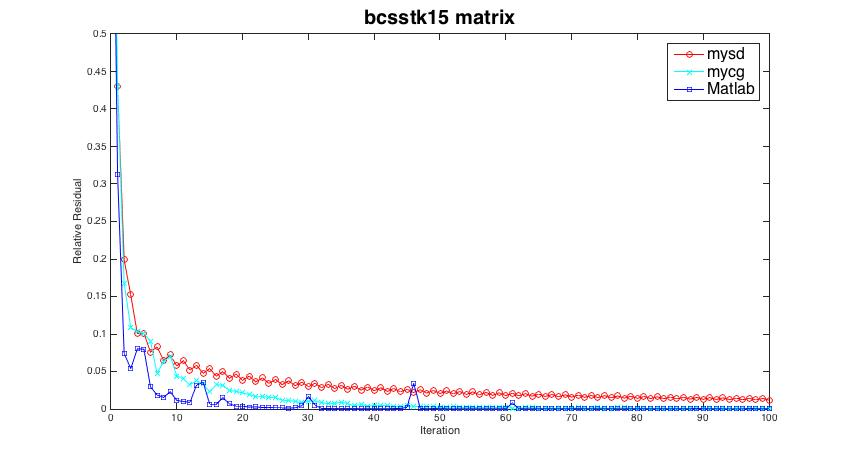
\includegraphics[width = 16cm, height = 6cm]{bc1.jpg}
      \end{figure}
      
      \begin{figure}[h]
      \centering
      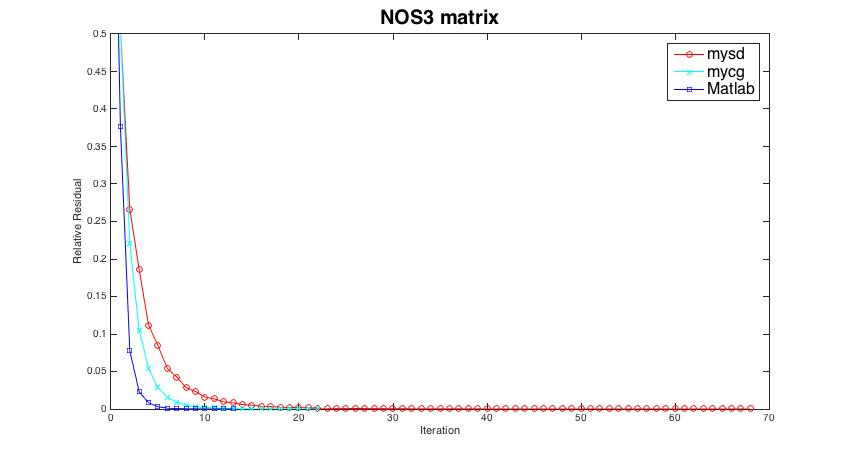
\includegraphics[width = 16cm, height = 6cm]{no2.jpg}
      \end{figure}
      
      
      
 \newline
 \newline
 \newline
 \newline
 \newpage
\subsection{Remarks and findings}
   \begin{enumerate}
       \item Both \textbf{bcsstk15} and \textbf{nos3} are tested with default starting point $x_0 = 0$ and with stopping tolerance 0.000001 and max iteration limits = 100000.
       \item For \textbf{bcsstk15}: All three implementation converge with some slight fluctuate during the process. mycg is better than mysd, and Matlab's cg is better than mine. All three methods' relative residual drop really quickly at the begining but requires a long time to meet our stopping criteria.
       \item For \textbf{nos3}:  All three implementation converge . mycg is better than mysd, and Matlab's cg is better than mine. And SD requires longer time than other two to meet the stopping criteria. 
      
   \end{enumerate}

\section{Nonsymmetric matrices}
\subsection{Results}
  Compare MR algorithm and GMRES algorithm with my self-written function and Matlab function gmres for GMRES algorithm.\\[1ex] 

\begin{figure}[h]
\centering
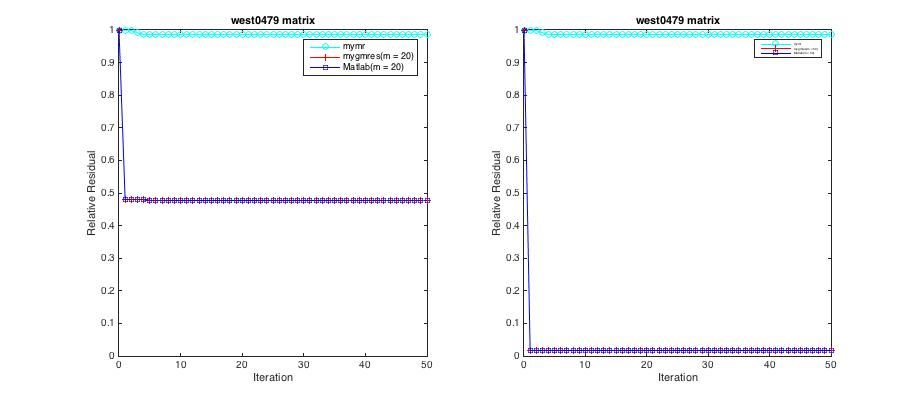
\includegraphics[width = \textwidth, height = 5.5cm]{west31.jpg}
\end{figure}
\begin{figure}[h]
\centering
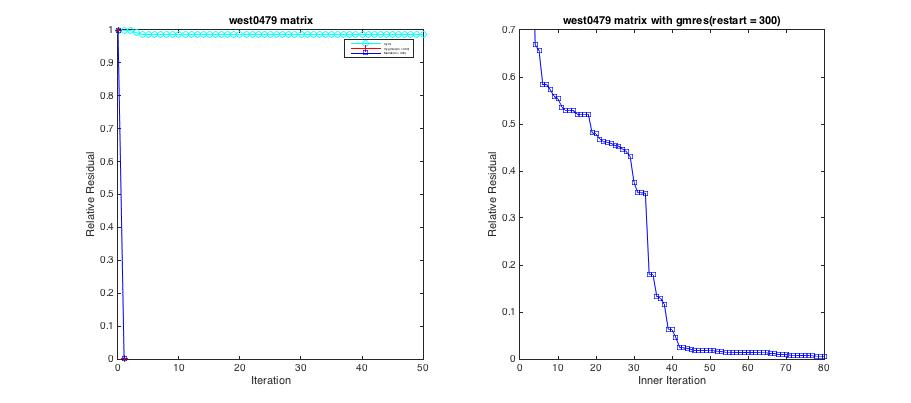
\includegraphics[width = \textwidth, height = 5.5cm]{west32.jpg}
\end{figure}

 \begin{figure}[h]
 \centering
      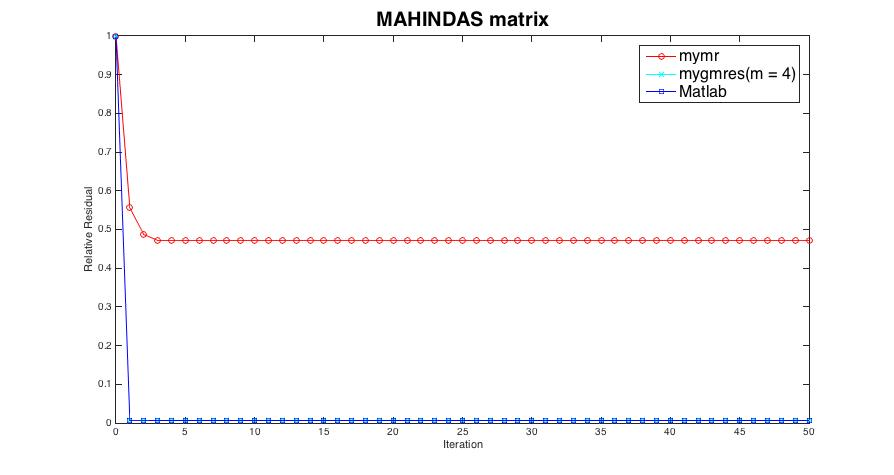
\includegraphics[width = 12cm, height = 5.5cm]{mah4.jpg}
      \end{figure}
\newpage
\subsection{Remarks and findings}
   \begin{enumerate}
       \item Both \textbf{west0479} and \textbf{mahindas} are tested with default starting point $x_0 = 0$ and with stopping tolerance 0.001 and max iteration limits = 5000. 
       \item For \textbf{west0479}, I tested restart = 20, 50 and 300. When restart is big enough, the algorithm will converge within one outer loop. But in this test, we can see it clearly that when restart = 20 and 50. The algorithm will not converge but the relative residuals will remain almost stationary in 5000 outer loop. 
       \item For \textbf{west0479}, we use Matlab's function gmres to plot each inner loop's performance with restart 300. It is easy to say that the algorithm went really well. 
       \item For \textbf{mahindas}, I tested restart  = 3,4, 5,6 and 100. When restart is no less than 6, the algorithm will converge with in one outer iteration. 
       \item Both matrices with MR algorithm are not converge to the optimal. It became stable after several steps. 
       \item When GMRES method with good setting of restart number, the algorithm performs better than MR method. But for these two matrices, both method did not perform very well. 
   \end{enumerate}

\section{Summary and Future topics}
\begin{enumerate}
    \item Normally, Conjugate Gradient Algorithm is superior to Steepest Gradient Algorithm when dealing with SPD system. CG converges faster than SG. To achieve a better performance of CG, we can add some preconditioning to the original Matrix.  
    \item For GMRES and MR method for solving nonsymmetric system, both algorithm did not perform well based on our test. Also, consider adding some preconditioning to it may get better performance. 
\end{enumerate}

\section{References}
\begin{enumerate}
    \item Professor Zhaojun Bai. Handout5 http://www.cs.ucdavis.edu/ bai/ECS231/
    \item Matlab help file from Mathworks.com http://www.mathworks.com/help/matlab/ref/gmres.html
    \item Professor Yousef Saad Unicersity of Minnesota. Handout: http://www-users.cs.umn.edu/~saad/Calais/PREC.pdf
\end{enumerate}


\newline
\newline
\newline
\newline
   
   
   
   
   
   

\newline
\newline
 - - - - - - - - - - - - - - - - - - - - - - - - - - - - - - - - - - - - - - - - - - - - - - - - - - - - - - - - - - - - - - - - - - - - - - 

$\quad$ Code and original plots: https://github.com/JaneJianshi/ECS231HW3
\end{document}

